\section{Background \& Prior Work}

% We assume general familiarity with the Web client-side architecture~\cite{shklarWebApplicationArchitecture2009}, protocols~\cite{HighPerformanceBrowsera}, and browser design~\cite{WebTechnologyDevelopers2025}. 
% Next, we overview important browser's framework concepts that web tracking techniques must work within (or around), outline the threat model of web tracking, and compare prior surveys in the field.

% \subsection{Threat Model of Web Tracking}
\label{sec:threat-model}

\para{Browser's Security Model: Context-Origin Boundaries.}
% A typical website is composed of a primary HTML document embedded with numerous inline or external resources fetched from a \textit{first-party} or \textit{third-party} web server. Upon inclusion, these resources can exhibit different behaviors depending on their type, context, and origin.
% % 
% By what is known as the \textit{Same-Origin Policy (SOP)}~\cite{mdnSameoriginPolicySecurity2024}, browsers tag and isolate content per origin, ensuring that code and data from different origins (or site groupings) cannot read, modify, or interfere maliciously with each other's state.
% % 
% Additionally, browsers label each context with the origin of its active document to enforce context boundaries and isolate each context in terms of the DOM and JavaScript runtime. By default, code in one context cannot arbitrarily interfere with a document in another context, especially if their origins differ.
The browser's context model denotes that every document runs in a container 
% (frame or window) 
that maintains its state (e.g., DOM, variables, scripts) separate from others, while the origin model associates the document with an origin determining the code’s privileges.
%
Thus, the browser uses both the origin and context to enforce policies---it isolates contexts from each other, and when an interaction is attempted, it checks the origins involved.
%
Under the \textit{Same-Origin Policy (SOP)}~\cite{mdnSameoriginPolicySecurity2024}, two contexts can interact freely only if they share the same origin.

\para{Entities (\autoref{fig:threat-model}).}
%%
% The threat model of web tracking comprises four main entities.
%
The \textbf{\textit{user}} is an individual accessing websites on the internet through their browser (also known as user agent~\cite{mdnUserAgentMDN2025}), seeking to keep their online behavior private. % and hence considered the \textit{victim}. % or at least under control.
%
The \textbf{\textit{browser}} mediates all interactions between the user and the web content, enforcing context-origin policies. % and providing necessary functionality for webpages.
%
The \textbf{\textit{first-party website}} is the webpage that the user directly browses for content.
%
It often includes resources from \textbf{\textit{third-parties}}, i.e., hosted on a different domain than the first-party website~\cite{mdnDomainMDNWeb2024}.


\begin{figure}[!ht]
    \centering
    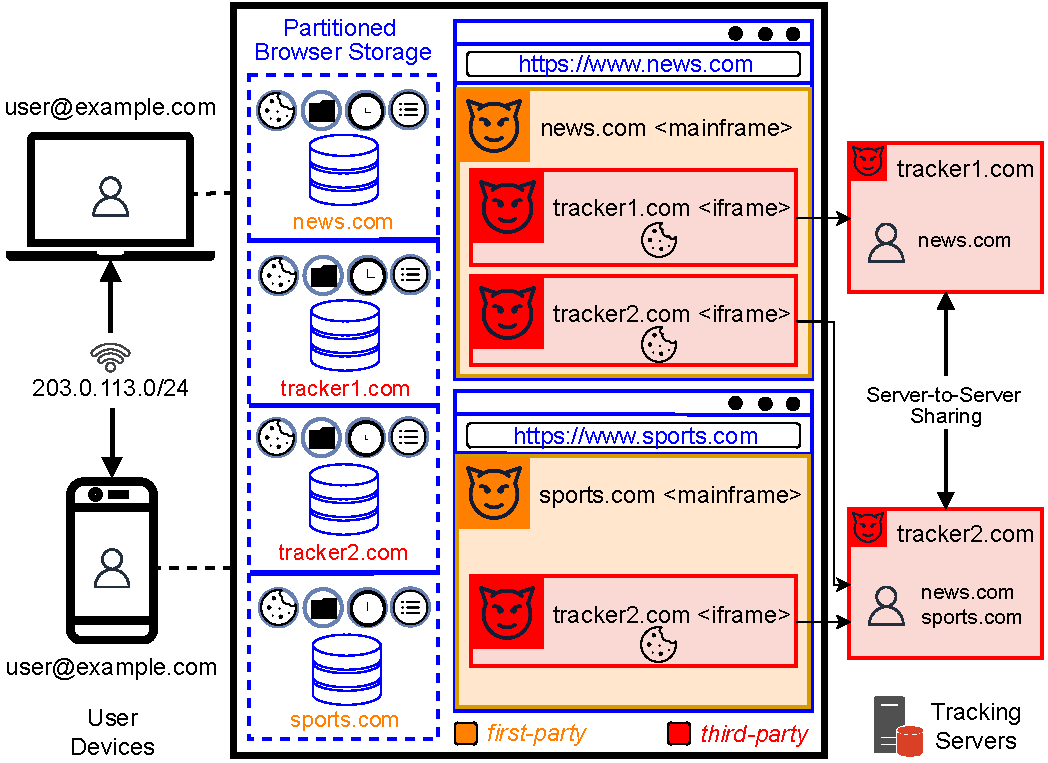
\includegraphics[width=\linewidth]{figures/threat-model.pdf}
    \caption{Conceptual overview of our threat model where \texttt{news.com} and \texttt{sports.com} are the first-party websites visited by the user from their personal device(s) and \texttt{tracker1.com} and \texttt{tracker2.com}  embedded third-parties.}
    \label{fig:threat-model}
\end{figure}



%%
\para{Adversary Goals.}
%
A tracker is any party whose goal is to collect user’s data in order to profile or identify the user’s behavior across one site (\textit{same-site tracking}), several sites (\textit{cross-site tracking}), across contexts (\textit{cross-context tracking}) on a given device
% (i.e., cross-app or cross-browser tracking) 
or across devices.
% (i.e., cross-device tracking).
%
% The primary goal is to persistently and uniquely label the user or their browser/device and to collect user data tied to that label, across navigations, sites, and over time, for profiling, analytics, or ad targeting.
%
Besides, a secondary goal may be to avoid detection and anti-tracking measures.

% for table:
% Author et al. or Title [cite], year, scope, (audience?), technique, defense, regulations, future directions, nb papers/refs
\begin{table*}[!ht]
    \centering
    \begin{tabular}{cccccccc}
    \toprule
    & & & \multicolumn{2}{c}{\textbf{Techniques}} & \multicolumn{2}{c}{\textbf{Defenses}}\\
    \textbf{Work} & \textbf{Year} & \textbf{Scope}& \textbf{Stateful} & \textbf{Stateless} & \textbf{Academic} & \textbf{Industrial} & \textbf{Regulations}\\
    \midrule
         Mayer and Mitchell~\cite{mayerThirdPartyWebTracking2012} & 2012 & Third-party tracking techniques and policy\\
         
         Bujlow et al.~\cite{bujlowSurveyWebTracking2017} & 2017 & Techniques and defenses\\
         
         Sanchez-Rola et al.~\cite{sanchez-rolaWebWatchingYou2017} & 2017 & Techniques and countermeasures\\
         
         Laperdrix et al.~\cite{laperdrix2020browser} & 2020 & Browser fingerprinting techniques and defenses\\
         
         % Schnitzler et al.~\cite{schnitzlerSoKManagingLongitudinal2021} & 2021 & \\ %out-of-scope (online service/social media data sharing)
         
         Rokicki et al.~\cite{rokickiSoKSearchLost2021} & 2021 & JS timers-based attacks\\
         
         Sprecher et al.~\cite{sprecherSoKAllNothing2022} & 2022 & Script inclusion and permissions\\
         
         Subramani et al.~\cite{subramaniSoKWorkeroundsCategorizing2022} & 2022 & Service workers-based attacks and mitigations\\
         
         Stafeev and Pellegrino~\cite{stafeevSoKStateKrawlers2024} & 2024 & Measurement crawlers and methodology\\
         
         Birrell et al.~\cite{birrellSoKTechnicalImplementation2024} & 2024 & Internet Privacy Regulations \\
         
         Rieder et al.~\cite{riederSoKDecadesWeb2026} & 2026 & Tracker detection (methodology measurements)\\
         
         \hline
         Ours & 2026 & Techniques, mitigations, and regulations & \pie{360} & \pie{360} & \pie{360} & \pie{360} &\\
     \bottomrule
    \end{tabular}
    \caption{Comparison overview to prior SoK and survey papers related to web tracking.}
    \label{tab:prior-sok-comparaisons}
\end{table*}

%%
\para{Adversary Capabilities.}
%
% A tracker's capabilities are shaped by the web's architecture and browser's security model discussed in ~\autoref{sec:background}.
%
% To achieve their goals, an adversary's capabilities can be explained in context of \textit{inclusion}, \textit{collection}, \textit{storage}, and \textit{sharing} of the user data, subject to the browser's context-origin restrictions discussed in~\autoref{sec:terminology}.
%
% The adversary is considered capable enough to track users either in presence of the browser-enforced policies discussed in~\autoref{sec:terminology} or by circumventing them.
%
\textbf{\textit{Inclusion} \symInclusion.}
%
A first-party tracker is assumed to directly monitor user activities within the top-level browsing context.
%
A third-party tracker could be embedded as an inline resource (e.g., image/script tag) within the mainframe by the first-party assuming trust delegation, an iframe with a separate context under its origin, or as a resource within a third-party iframe.
%
\textbf{\textit{Execution} \symExecution.}
%
A tracker aims to collect user data through available browser features 
% by executing JavaScript code 
within the context where it is embedded. 
%
A script's execution privileges are tied to its context’s origin---implying that it always ``acts as'' whatever origin its document has.
%
% As a result, when an external script is included in a document from an origin different from the including document's origin, the browser does not enforce any origin-based restriction.
%
% The script executes with full privileges of the context that included it---it can access the including page’s DOM, make network requests as that page, read and set storage of that page, and generally do anything the page’s own scripts could do.
%
By including external scripts, the webpage implicitly declares that it trusts that code with its own origin’s privileges~\cite{TrackingPreventionWebKit2020}.
%
\textbf{\textit{Storage} \symStorage.}
%
Trackers may also read, write, or modify data in the user's browser storages,
% such as \texttt{localStorage}, \texttt{sessionStorage}, \texttt{indexedDB},
which are partitioned by origin, as well as the cookie jar, which is scoped by domain (and path) rather than the full origin.
%
Stored data can be accessed by the tracker in subsequent visits to either the same site or a different site.
%
Scripts from one origin cannot read or write to another origin’s storage.
%
Because cookies are not origin-partitioned, third-party scripts included in the main execution context can read and write first-party cookies.
% (e.g., using \texttt{document.cookie} or CookieStore API).
%
\textbf{\textit{Sharing} \symSharing.}
%
To share collected data with its own servers or a partner's, trackers can initiate network requests including the user data in one of four ways: (1)~as a URL query parameter, (2)~request payload, (3)~request header, or (4)~through HTTP cookies.
%
% Approaches 1-3 require tracking scripts to explicitly include user data, whereas HTTP cookies associated with the tracker's domain are automatically included in all requests to the tracker's server. % (e.g., setting a custom request header for tracking).
%
% In case of 4, browsers automatically attach the previously set tracker's cookies with the requests sent to the tracker’s domain as a request header, even if that request originates in a first-party context.
%
\textbf{\textit{Observation} \symObservation.}
%
A tracker present outside the browser can also passively observe and analyze network traffic from the user's browser or device.
%%
% We use this threat model to understand different web tracking mechanisms and their evolution over time.


\para{Related Systematization Work.}
%
Over the years, the web tracking community has produced a considerable amount of findings.
%
Unfortunately, these have largely remained scattered across disjoint works making it difficult to draw connections between related techniques, assess the state of the field, and identify future research directions.
%
Our SoK addresses these by providing the most recent, systematic, and unified view of the evolution of all known tracking techniques and their research-, industry-, and community-based defense mechanisms in parallel to major EU and US regulatory and compliance changes.
%
Prior survey and SoK papers in the space (see comparison overview in~\autoref{tab:prior-work}) have only partially covered such aspects; being too high-level~\cite{ermakova2018web,bujlowSurveyWebTracking2017}, too narrowly-focused on specific tracking mechanisms~\cite{laperdrix2020browser,rokickiSoKSearchLost2021}, research measurement methodologies~\cite{stafeevSoKStateKrawlers2024,riederSoKDecadesWeb2026}, or regulations exclusively~\cite{birrellSoKTechnicalImplementation2024}, or too old and outdated by newer techniques, defenses, and policies that appeared in recent years~\cite{mayerThirdPartyWebTracking2012,sanchez-rolaWebWatchingYou2017}.
%
% We refer to~\autoref{tab:prior-work} for a comparison of the scope of our SoK with prior work.